\documentclass{article}
\usepackage{v-problem}
\vgeometry

\begin{document}
\vtitle[KINEMATICS]

\def\pn{03}
\def\book{Irodov}
\def\page{13}
\def\gdrive{https://drive.google.com/drive/folders/1SlBEDIHXM9BURM7e5NXAWJpv8zaMnSCp?usp=share_link}

\def\question{
Three points are located at the vertices of an equilateral triangle whose side equals $a$. They all start moving simultaneously with velocity $v$ constant in modulus, with the first point heading continually for the second, the second for the third, and the third for the first. How soon will the points converge?
}

\def\option{
}

\def\diagram{
\begin{center}
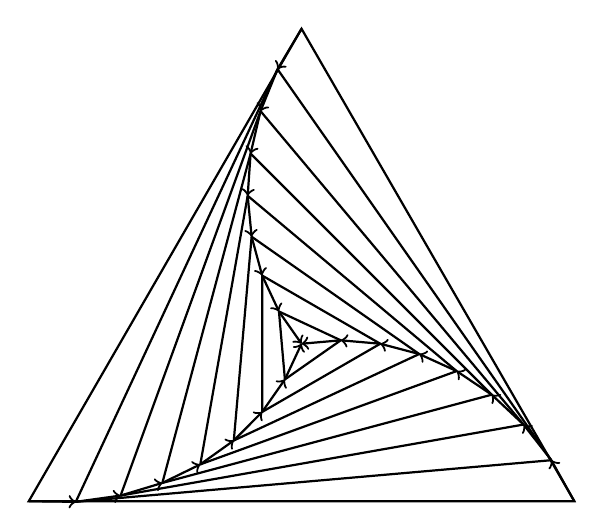
\begin{tikzpicture}
[thick]
\foreach \angle/\side in {0/4, 5/3.5, 10/3, 15/2.5, 20/2, 25/1.5, 30/1, 35/0.5}{
	\draw[rotate=\angle] (-30:\side)--(90:\side)--(210:\side)--cycle;
	\draw[->] (-30+\angle:\side)--(-30+\angle+5:\side-0.5);
	\draw[->] (90+\angle:\side)--(90+\angle+5:\side-0.5);
	\draw[->] (210+\angle:\side)--(210+\angle+5:\side-0.5);
}
\tzdots*<0, 3pt>(-30:4)(90:4)(210:4);(6pt)
\end{tikzpicture}
\end{center}
}

\vspace*{\fill}
\begin{tikzpicture}
	\node[qnumber] (n) at (0, 0)[scale=2] {$\pn.$};
	\node[question] (q) [right=2mm of n.east] {\question};
	\tzline[divider]<-0.125, 0> (q.north west)(q.south west);
	\node[format] (f) at  (q.south east){[\book \quad \page]};
	\node[diagram] (d) [below=0.5cm of q.south] {\diagram};
	\node[option] (o) [below=0.1cm of d.south] {\option};
\end{tikzpicture}	
\vspace*{\fill}
\pagebreak
\vtitle[SOLUTION]
\begin{center}
\begin{tikzpicture}
[thick]
\def\side{3.5}
	\draw[dashed] (-30:\side)--(90:\side)--(210:\side) node[midway, left]{$l$} --cycle;
	\draw[->] (-30:\side)--+(120:\side-2) node[right]{$\vec{v}_2$};
	\draw[->] (90:\side)--+(240:\side-2) node[left]{$\vec{v}_3$};
	\draw[->] (210:\side)--+(0:\side-2) node[below]{$\vec{v}_1$} coordinate(V1);
	
	
	
	\draw[->, PINKD] (210:\side)--+(60:\side-2) node[right]{$\vec{v}_1\cos60^\circ$} coordinate(V13);
	
	\draw[->, PINKD] (210:\side)--+(-30:\side-2) node[right, below]{$\vec{v}_1\sin60^\circ$} coordinate(V1P3);
	
	\tzanglemark(V1)(210:\side)(V13){$60^\circ$}(15pt)
	

\tzdots*(-30:\side)(90:\side)(210:\side);(6pt)
\end{tikzpicture}
\end{center}

\begin{align*}
-\dfrac{\d{l}}{\d{t}} &= | \vec{v}_{31} |_{\texttt{along the path}}\\
-\dfrac{\d{l}}{\d{t}} &= v+v\cos(60^\circ)
\end{align*}
\pagebreak

\addtolength{\jot}{3ex}
\begin{align*}
-\dfrac{\d{l}}{\d{t}} &= v+v\cos(60^\circ)\\
-\int_a^0 \d{l} &= \dfrac{3v}{2}\int_0^t \d{t}\\
a &= \dfrac{3v}{2} t\\
t &= \dfrac{2a}{3v} \ans
\end{align*}

\pagebreak
\vspace*{\fill}
\begin{center}
	\fbox{\qrcode[height=2cm]{\gdrive}}
\end{center}
\vspace*{\fill}
\end{document}
